\documentclass{article}
\usepackage{color}
\usepackage{tikz}
\usepackage{float}
\usepackage{tabularx}
\usepackage{amsmath}
\usepackage{amssymb}
\usepackage{listings}
\usepackage{enumitem}
\usepackage{syntax}
\usepackage{csquotes}
\usepackage[backend=biber]{biblatex}
\addbibresource{references.bib}

\usepackage{tikz}
\usetikzlibrary{automata,positioning}

\definecolor{dkgreen}{rgb}{0,0.6,0}
\definecolor{gray}{rgb}{0.5,0.5,0.5}
\definecolor{mauve}{rgb}{0.58,0,0.82}


\lstset{frame=tb,
  numbers=left,
  stepnumber=1,
  language=Java,
  aboveskip=3mm,
  belowskip=3mm,
  showstringspaces=false,
  columns=flexible,
  basicstyle={\small\ttfamily},
  numberstyle=\color{gray},
  keywordstyle=\color{blue},
  commentstyle=\color{dkgreen},
  stringstyle=\color{mauve},
  breaklines=true,
  breakatwhitespace=true,
  tabsize=2,
  moredelim=**[is][\color{red}]{@}{@},
}

\setlength{\grammarindent}{12em}

%\renewcommand{\lstlistingname}{Algorithm}
%\newcommand{\tablerow}[4]{ #1 & #2 & #3 & #4\\}
\newcommand{\n}[0]{\\[\baselineskip]}
%\newcommand{\qa}[2]{\textbf{Q:} #1 \\ \textbf{A:} #2}
%\newcommand{\argument}[4]{\textbf{#1:} #2 \\ \textbf{#3:} #4}

\title{CS4303 Particle Command Report}
\author{Sizhe Yuen}

\begin{document}

\maketitle

\section{Introduction}
In this practical we were tasked to implement the video game \textit{Particle Command}, which is a variant on missile command where the particles are blasted away from the explosion rather than being destroyed. In my game, I have implemented all the features in the practical specifications as well as some additional features.
\n
TODO RUN INSTRUCTIONS

\section{Game features}

\subsection{Basic}
\subsubsection*{Meteors}
The particles falling are implemented in the \texttt{Meteor} class. They spawn from a random location at the top of the screen and have a random initial velocity. This initial random velocity goes from \texttt{-2f} to \texttt{2f} in the x direction and from \texttt{0} to \texttt{3f} in the y direction. The random y velocity makes some particles come down faster than others to make the game a bit more interesting. They do not have a random negative y velocity because all particles not in the screen are destroyed. 

\subsubsection*{Cities}
There are five locations where the cities are placed on the ground of the play area. These are static and do not change. This was done for simplicity and a fair balance so there are not occasional games where the cities are very far away, making the game more difficult. 

\begin{figure}[H]
\centering
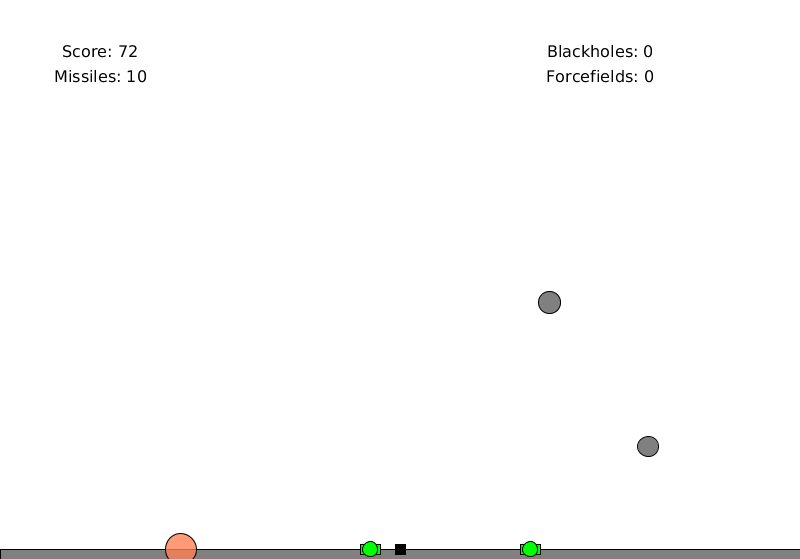
\includegraphics[width=1\textwidth, keepaspectratio]{imgs/Meteors.png}
\caption{Meteors falling from the sky. The one on the left has hit the ground and caused an explosion. Remaining cities can be seen in green.}
\end{figure}

\subsubsection*{Explosions}
All particles can create explosions when they are destroyed as it is an abstract method all \texttt{Particle} subclasses must implement. In my game, both the meteors and player missiles create explosions. The explosion radius is based off of the particle's initial radius, increasing with each time step until they've reach the end of their lifespan. Any particles caught in the blast radius are blown away with an \texttt{Explosive} force. 

\subsubsection*{Player missiles}
The player missiles fire from the center of the ground. Their velocity is normalised so it takes a bit of planning to properly defend the cities that are further away. The missile explode either when they reach their destination - the position of the mouse cursor when the missile was fired - or when they collide with a meteor during their trajectory. 


\subsubsection*{Waves}
\begin{figure}[H]
\centering
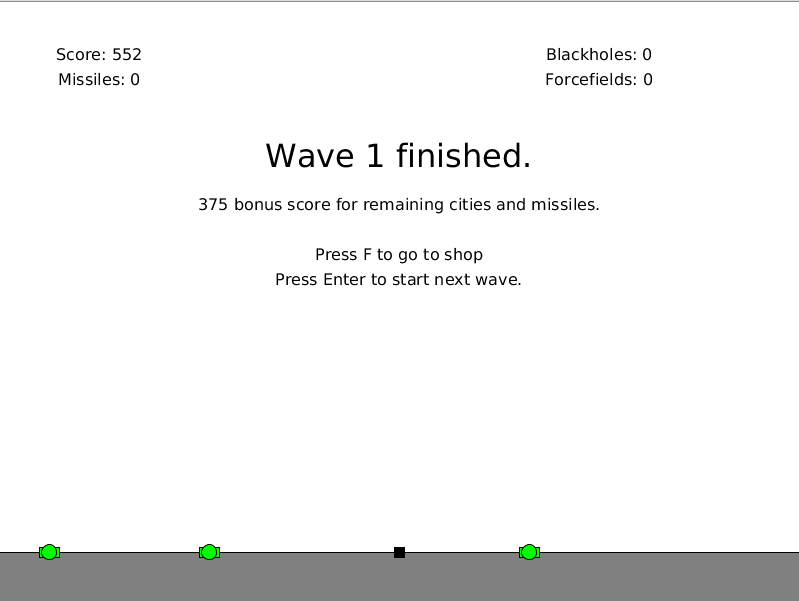
\includegraphics[width=1\textwidth, keepaspectratio]{imgs/WaveFinished.png}
\end{figure}
The game is organised into waves. At the beginning of each wave, the number of missiles the player has is increased. Each wave has increasing difficulty as more meteors are spawned. Every few waves, the player is rewarded with a black hole or forcefield to help them survive. However, every few waves a bomber also comes which makes the game more difficult.


\subsection{Extension}

\subsubsection*{Split into child meteors}
To make the game more difficult, the extension for splitting meteors into child meteors is also implemented. Meteors that are larger than a certain radius have a chance to split into 2 or more child meteors. As the player goes into higher levels, the number of child meteors that spawn is increased. 

\subsubsection*{Bombers}
In addition to splitting the meteors, bombers that drop "bombs" are also implemented in the game. These bombers fly across the screen and drop "bombs" that are much heavier than normal meteors. They are also given an initial downwards velocity to make them fly faster towards the player's cities.
\n
In the code, the bombs are implemented as meteors but drawn with a darker colour. This is because apart from flying faster to the ground they are the same as regular meteors. 

\subsubsection*{Black holes}
To add the force of gravitational attraction to the game, I added a special missile that player's can shoot which would create a black hole. The black holes apply gravitational attraction to all meteors on screen and because they are intentionally much heavier than the meteors, most will be sucked into the black hole and destroyed. Meteors that are further away may be affected less.
\n
The black holes only last for a short while before disappearing. This means that if a meteor was being accelerated towards it but did not get sucked in, even though it no longer has the gravitational force acting on it, it may have been accelerated to a very fast velocity and crash down onto a player's city. This makes the use of black holes more strategic and a double edged sword if used improperly. 
\subsubsection*{Forcefield}
Unlike explosions, forcefield use a different kind of force to repel particles which makes them a more global and powerful tool to deflect meteors compared to missiles. Instead of applying an explosive force to knock the meteors away, forcefields use the opposite force of gravitational attraction. The meteors are repulsed away from the forcefield by multiplying the force of gravitational attraction by -1. 
\n
The button for using forcefields is the middle mouse button.



\subsubsection*{Shop}
To allow the player the ability to use more of these special particles, I have added a little shop screen for players to spend score to purchase extra black holes, forcefields and missiles. Because these cost score to buy, the player must choose between keeping their score high, or using it to ensure they don't lose in the next round. 


\section{Design}


\subsection{Physics}


\subsection{Collision}
 

\subsection{State management}
To split the game up into different states such as start of game, end of wave, shop etc, I've implemented each state as its own separate class and made the game change states like a state machine. I got this idea from the state chapter of the book Game Programming Patterns (http://gameprogrammingpatterns.com/state.html).
\n
The idea is that on each \texttt{update()} or \texttt{handleInput()} step, the current state will return what the next state should be. For example if the game is currently in the \texttt{EndOfWaveState} and it gets the enter key - the key to start the next wave - it returns a \texttt{PlayingState} with the next wave of enemies. This allows each state to only keep track of themselves and handle everything that happens in the state within their own class. 
\n
\begin{figure}[H]
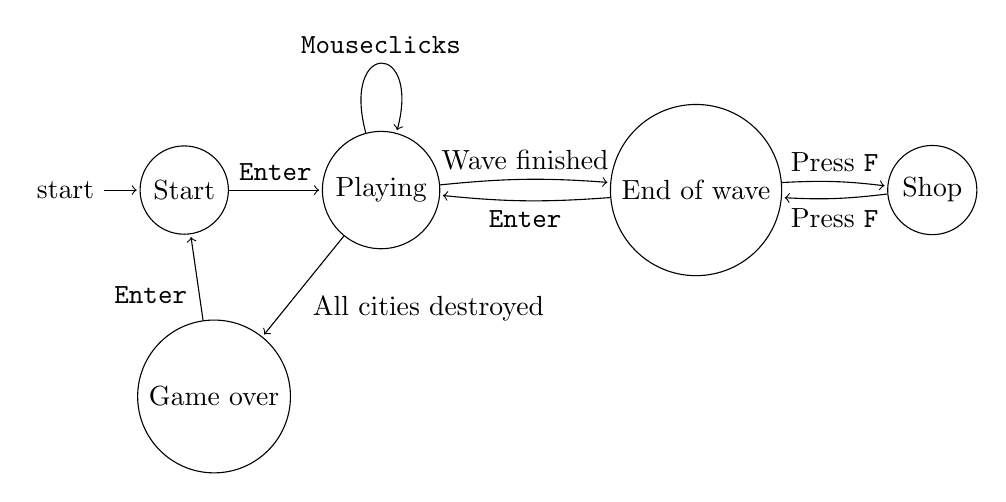
\begin{tikzpicture}[shorten >=1pt,node distance=3cm,on grid,auto]
		\node[state,initial] (Start) {Start};
		\node[state] (Playing) [right=of Start, xshift=-0.5cm] {Playing};
		\node[state] (EndOfWave) [right=of Playing, xshift=1cm] {End of wave};
		\node[state] (Shop) [right=of EndOfWave] {Shop};
		\node[state] (GameOver) [below left=of Playing, yshift=-0.5cm] {Game over};
		
		\path[->]
		(Start) edge node {\texttt{Enter}} (Playing)
		(Playing) edge [loop above] node {\texttt{Mouseclicks}} (Playing)
				  edge[above, bend left=5] node {Wave finished} (EndOfWave)
				  edge node {All cities destroyed} (GameOver)
		(EndOfWave) edge[below, bend left=5] node {\texttt{Enter}} (Playing)
					edge[above, bend left=5] node {Press \texttt{F}} (Shop)
		(Shop) edge[below, bend left=5] node {Press \texttt{F}} (EndOfWave)
		(GameOver) edge node {\texttt{Enter}} (Start);
					
\end{tikzpicture}
\caption{State machine of the game.}
\end{figure}
\printbibliography

\end{document}